\documentclass[11pt,a4paper]{article}
\usepackage[utf8]{inputenc}
\usepackage[T1]{fontenc}
\usepackage[romanian]{babel}
\usepackage[margin=1.9cm]{geometry}
\usepackage{amsmath,amssymb}
\usepackage{enumitem}
\usepackage{parskip}
\usepackage{tikz}
\usetikzlibrary{arrows.meta,positioning,calc}
\setlist{nosep, topsep=2pt, itemsep=2pt, leftmargin=1.3em}
\setlength{\parskip}{3pt}
\pagestyle{empty}

\begin{document}
\begin{center}
{\large\bfseries MODEL DE ANTRENAMENT --- SAE}\\[1pt]
{\small (subiect generat pentru autoevaluare, nu e biletul oficial de examen)}
\end{center}
\vspace{0.1cm}

\begin{enumerate}[leftmargin=1.4em]

\item Fie sistemul din figură ($T_e=0.1$s), unde $G(s)=1/(s(s+5))$.

\begin{center}
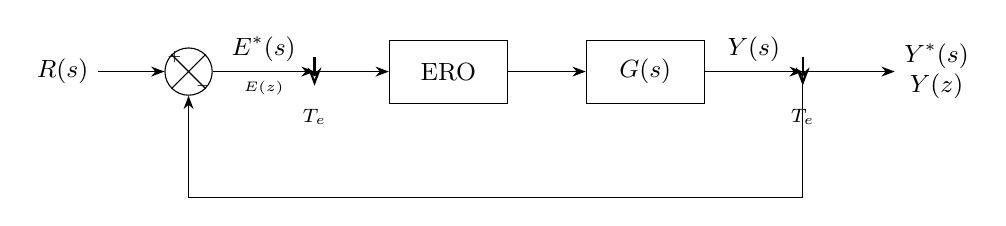
\begin{tikzpicture}[>=Stealth, font=\small]
\node (R) at (0,0) {$R(s)$};
\node[draw,circle,minimum size=6mm] (sum) at (1.6,0) {};
\draw (sum.north west) -- (sum.south east) (sum.north east) -- (sum.south west);
\node at ($(sum)+(-0.18,0.18)$) {\tiny$+$};
\node at ($(sum)+(0.18,-0.18)$) {\tiny$-$};

\coordinate (sw) at (3.2,0);
\node[draw,minimum width=15mm,minimum height=8mm] (ero) at (4.9,0) {ERO};
\node[draw,minimum width=15mm,minimum height=8mm] (g) at (7.4,0) {$G(s)$};
\coordinate (swY) at (9.4,0);
\node (Yout) at (11.1,0) {$\begin{matrix}Y^*(s)\\ Y(z)\end{matrix}$};

\draw[->] (R) -- (sum);
\draw[->] (sum) -- (sw) node[midway,above]{$E^*(s)$} node[midway,below]{\tiny$E(z)$};
\draw[-{Stealth[open]},thick] ($(sw)+(0,0.18)$) -- ++(0,-0.36);
\node[below] at ($(sw)+(0,-0.35)$) {\scriptsize $T_e$};
\draw[->] (sw) -- (ero);
\draw[->] (ero) -- (g);
\draw[->] (g) -- (swY) node[midway,above]{$Y(s)$};
\draw[-{Stealth[open]},thick] ($(swY)+(0,0.18)$) -- ++(0,-0.36);
\node[below] at ($(swY)+(0,-0.35)$) {\scriptsize $T_e$};
\draw[->] (swY) -- (Yout);

\draw[->] (swY) |- ++(0,-1.6) -| (sum);
\end{tikzpicture}
\end{center}

\begin{enumerate}[label=\alph*)]
\item Să se determine funcția de transfer a sistemului în circuit închis folosind metoda de integrare a trapezului. (1p)
\item Să se determine pentru ce mărime de intrare sistemul prezintă eroare staționară finită. (0.5p)
\item Să se determine și să se reprezinte grafic răspunsul sistemului la mărimea de intrare impuls unitar Dirac. (1p)
\end{enumerate}
\emph{Pentru punctele b) și c) se folosesc rezultatele de la punctul a).}

\item Se consideră un sistem cu reacție negativă unitară, în care funcția de transfer a sistemului în circuit deschis este de următoarea formă ($T_e=1$s) (2p):
$$G_d(z)=\frac{0,2z+0,07}{z^2-0,5z+0,05}$$
Să se reprezinte caracteristicile amplitudine-pulsație și fază-pulsație.

\item Se consideră un sistem cu reacție negativă unitară, în care funcția de transfer a sistemului în circuit deschis este de următoarea formă ($T_e=1$s) (1.5p):
$$G_d(z)=\frac{k(0,13z+0,02)}{z^2-0,39z+0,007}$$

Determinați:
\begin{enumerate}[label=\alph*)]
\item Nr. de ramuri ale locului rădăcinilor; de unde încep ramurile și unde se termină. (0.2p)
\item Porțiunea de pe axa reală care aparține locului rădăcinilor. (0.15p)
\item Nr. de asimptote, unghiul pe care-l fac cu axa reală și punctul unde se întâlnesc pe axa reală. (0.15p)
\item Punctele de ramificație. (0.5p)
\item Verificați dacă locul rădăcinilor descrie un cerc. Trasați locul rădăcinilor. (1p)
\end{enumerate}

\item Se consideră funcția de transfer a unui sistem în circuit închis:
$$G_0(z)=\frac{0,02z+0,02}{z^2-1,49z+0,54}$$
\begin{enumerate}[label=\alph*)]
\item Să se determine modelul cu variabile de stare în forma complet controlabilă (demonstrație). (1p)
\item Plecând de la modelul cu variabile de stare (matricele sistemului) să se determine dacă sistemul este observabil (se va calcula matricea $Q$). (1p)
\end{enumerate}

\item Se consideră funcția de transfer a unui sistem în circuit închis:
$$G(z)=\frac{z^2-1,39z+0,52}{z^2-1,43z+0,49}$$
\begin{enumerate}[label=\alph*)]
\item Să se determine modelul cu variabile de stare în forma complet observabilă (demonstrație). (1p)
\item Plecând de la modelul cu variabile de stare să se realizeze schema bloc. (1p)
\end{enumerate}

\end{enumerate}

\textbf{Teorie:}
\begin{enumerate}[leftmargin=1.4em]
\item Transformarea planului $s$ în planul $z$ (porțiunea 1-2).
\item Să se prezinte schema bloc funcțională pentru un sistem de reglare numeric.
\item Care sunt etapele în procesul de conversie analog-numerică?
\item Care sunt elementele specifice unui sistem numeric?
\item Cum este reprezentat într-o schemă bloc un eșantionor ideal?
\end{enumerate}

\vspace{0.2cm}
\small Toate subiectele teoretice valorează 1 punct.

\end{document}
